\documentclass{article}
\usepackage[pdftex,
        colorlinks=true,
        urlcolor=rltblue,       % \href{...}{...} external (URL)
        filecolor=rltgreen,     % \href{...} local file
        linkcolor=rltred,       % \ref{...} and \pageref{...}
        pdftitle={Phys 20 Lab 5},
        pdfauthor={Chris Dudiak},
        pdfproducer={pdfLaTeX},
        pagebackref,
        pdfpagemode=None,
        bookmarksopen=true]{hyperref}
\usepackage{color}
\usepackage{pdfpages}
\usepackage{graphicx}
\usepackage{mathtools}
\usepackage{placeins}
\usepackage{listings}
\usepackage{verbatim}
\definecolor{rltred}{rgb}{0.75,0,0}
\definecolor{rltgreen}{rgb}{0,0.5,0}
\definecolor{rltblue}{rgb}{0,0,0.75}


\begin{document}

\title{Phys 20 Lab 5 - Grapefruit Experiment}
\author{Chris Dudiak}
\date{\today}
\maketitle

\section{Part 1 - Optimal Angle}

By maximizing the distance equation, $d = v_0 Cos[\theta] t$ subject to $v_0 Sin[\theta] - .5 *9.8 * t^2 = 0$ with $t > 0$, we find the 
optimal firing angle is 45 degrees. 

To solve for the velocity required to reach PCC at 1000m, we solve for $v_0$ when the heights when y = 0 i.e. when 
${{v_0*Sin[\theta]*x} \over {v_0 * Cos[\theta]}} - .5 * 9.8 * {{x} \over {v_0 * Cos[\theta]}}^2 = 0$. This gives us an initial velocity of 98.9949m/s. This
corresponds to 70m/s in the x and 70m/s in the y direction.

\section{Part 2 - No Drag}
Using Mathematica's NDSolve, with initial conditions $x[0] = 0, y[0] = 0, x'[0] = 70, y'[0] = 70$ and parameters $x''[t] = 0, y''[t] = -9.8$
we verify the shot hits the target.

\begin{figure}[h!]
	\centering
	\includegraphics[scale=.6]{"trajectory"}
	\caption{Trajectory for $\theta = 45deg, v_0 = 99.9949m/s$}
\end{figure} 
\FloatBarrier

Plotting several angles with the same initial velocity at once, we can see how the angle affects the shot. The angles vary by 5 degrees and 
have an opacity scaled to how long they are in the air.

\begin{figure}[h!]
	\centering
	\includegraphics[scale=.6]{"trajectories"}
	\caption{Trajectories for  $v_0 = 99.9949m/s$ at angles from 0 to $\pi/2$}
\end{figure} 
\FloatBarrier

We can see that increasing the angle up to 45 degrees improves the distance but after that, increasing the angle further reduces the distance.

\section{Part 3 - Drag}

If the grapefruit has a mass of .5kg and a radius of .05m then the grapefruit will have the following trajectory in the presence of drag:

\begin{figure}[h!]
	\centering
	\includegraphics[scale=.6]{"drag"}
	\caption{Trajectory for $\theta = 45deg, v_0 = 99.9949m/s$ with Drag}
\end{figure} 
\FloatBarrier

As we can see, the grapefruit only reaches about 330m, quite far from its 1000m target.

\section{Part 4 - Guess the Correct Answer}
By varying the angle and the velocity accordingly, we can attempt to guess a valid solution in the presence of drag.
\begin{figure}[h!]
	\centering
	\includegraphics[scale=.6]{"dragGuess1"}
	\caption{Trajectory for $\theta = 45deg, v_0 = 800m/s$}
\end{figure} 
\begin{figure}[h!]
	\centering
	\includegraphics[scale=.6]{"dragGuess2"}
	\caption{Trajectory for $\theta = 22.5deg, v_0 = 800m/s$}
\end{figure} 
\begin{figure}[h!]
	\centering
	\includegraphics[scale=.6]{"dragGuess3"}
	\caption{Trajectory for $\theta = 20deg, v_0 = 780m/s$}
\end{figure} 
\FloatBarrier

We see that 20Degrees with a $v_0 = 780m/s$ hits our target well. Similarly to the without drag case, we can vary the angle for this velocity
to see what curves result. 

\begin{figure}[h!]
	\centering
	\includegraphics[scale=.6]{"dragTrajectories"}
	\caption{Trajectories for  $v_0 = 780m/s$ at angles from 0 to $\pi/2$}
\end{figure} 
\FloatBarrier

We can see that increasing the angle up to 20 degrees improves the distance but after that, increasing the angle further reduces the distance.

Finally, we can see there are a family of curves that result in the same distance, but with very different initial conditions.

\begin{figure}[h!]
	\centering
	\includegraphics[scale=.6]{"1000drag"}
	\caption{Trajectories that Reach 1000m with Drag}
\end{figure} 
\FloatBarrier

\section{Part 5 - Exact Solutions}

Finally, we can make a series of functions to calculate the exact results using NDSolve.
\begin{verbatim}
	init[v0_, th_] := {x[0] == 0, y[0] == 0, x'[0] == v0*Cos[th], y'[0] == v0*Sin[th]}

	rule[v0_, th_] := NDSolve[Join[eqsD, init[v0, th]], {x, y}, {t, 0, 100}][[1]]

	xxFunc[t_, v0_, th_] := x[t] /. rule[v0, th]

	yyFunc[t_, v0_, th_] := y[t] /. rule[v0, th]

	time[v0_, th_] := t /. FindRoot[yyFunc[t, v0, th], {t, 20}]

b)

range[v0_, th_] := xxFunc[time[v0, th], v0, th]

c)

initVel[th_, rng_] := Module[{nextRng = 0},
  For[v = 1, nextRng < rng, v = v + 1, 
   nextRng = range[v + 1, th];
   If[nextRng > rng, Return[v + 1]]]]

d)

initAngle[rng_] := 
 Module[{prevVel = initVel[Pi/180, rng], nextVel = 0},
  For[th = 5*Pi / 180, th < Pi/2, th = th + Pi /180;
   nextVel = initVel[th + Pi/180, rng];
    If[prevVel <= nextVel, Return[th + Pi/180]];
   prevVel = nextVel]]
\end{verbatim}

The NDSolve takes a velocity and an angle and calculates the functions for the general drag equations and the initial conditions defined by the input.
We can make x and y position functions of t by evaluating on these rules. Then the time in the air, as a function of the parameters, is simply the point
at t not equal to 0 where yyFunc has a height of 0. The range for this value is simply xxFunc evaluated at this time and initial conditions. The initial
velocity is found by increasing the velocity until for a given angle until we get passed our desired range. For the initial angle, we simply move from
5 degrees to 90 degrees 1 degree at a time looking for an angle that requires less velocity than the next higher angle. This will get us a lowest velocity
since up to some angle (roughly 20degrees) we need less velocity to reach 1000m, but after this point, the drag forces cause us to need more velocity.
Using this function, we find at range 1000m, we need an angle of ${2 \pi \over 15}$ or 24 degrees. This could be made more accurate by taking smaller
step sizes in both velocity and angle, but this increases the run time.

\section{Code and Info}

\subsection{Code}
Code for this week's set is appended at the end of the file as a pdf version of the Mathematica code.
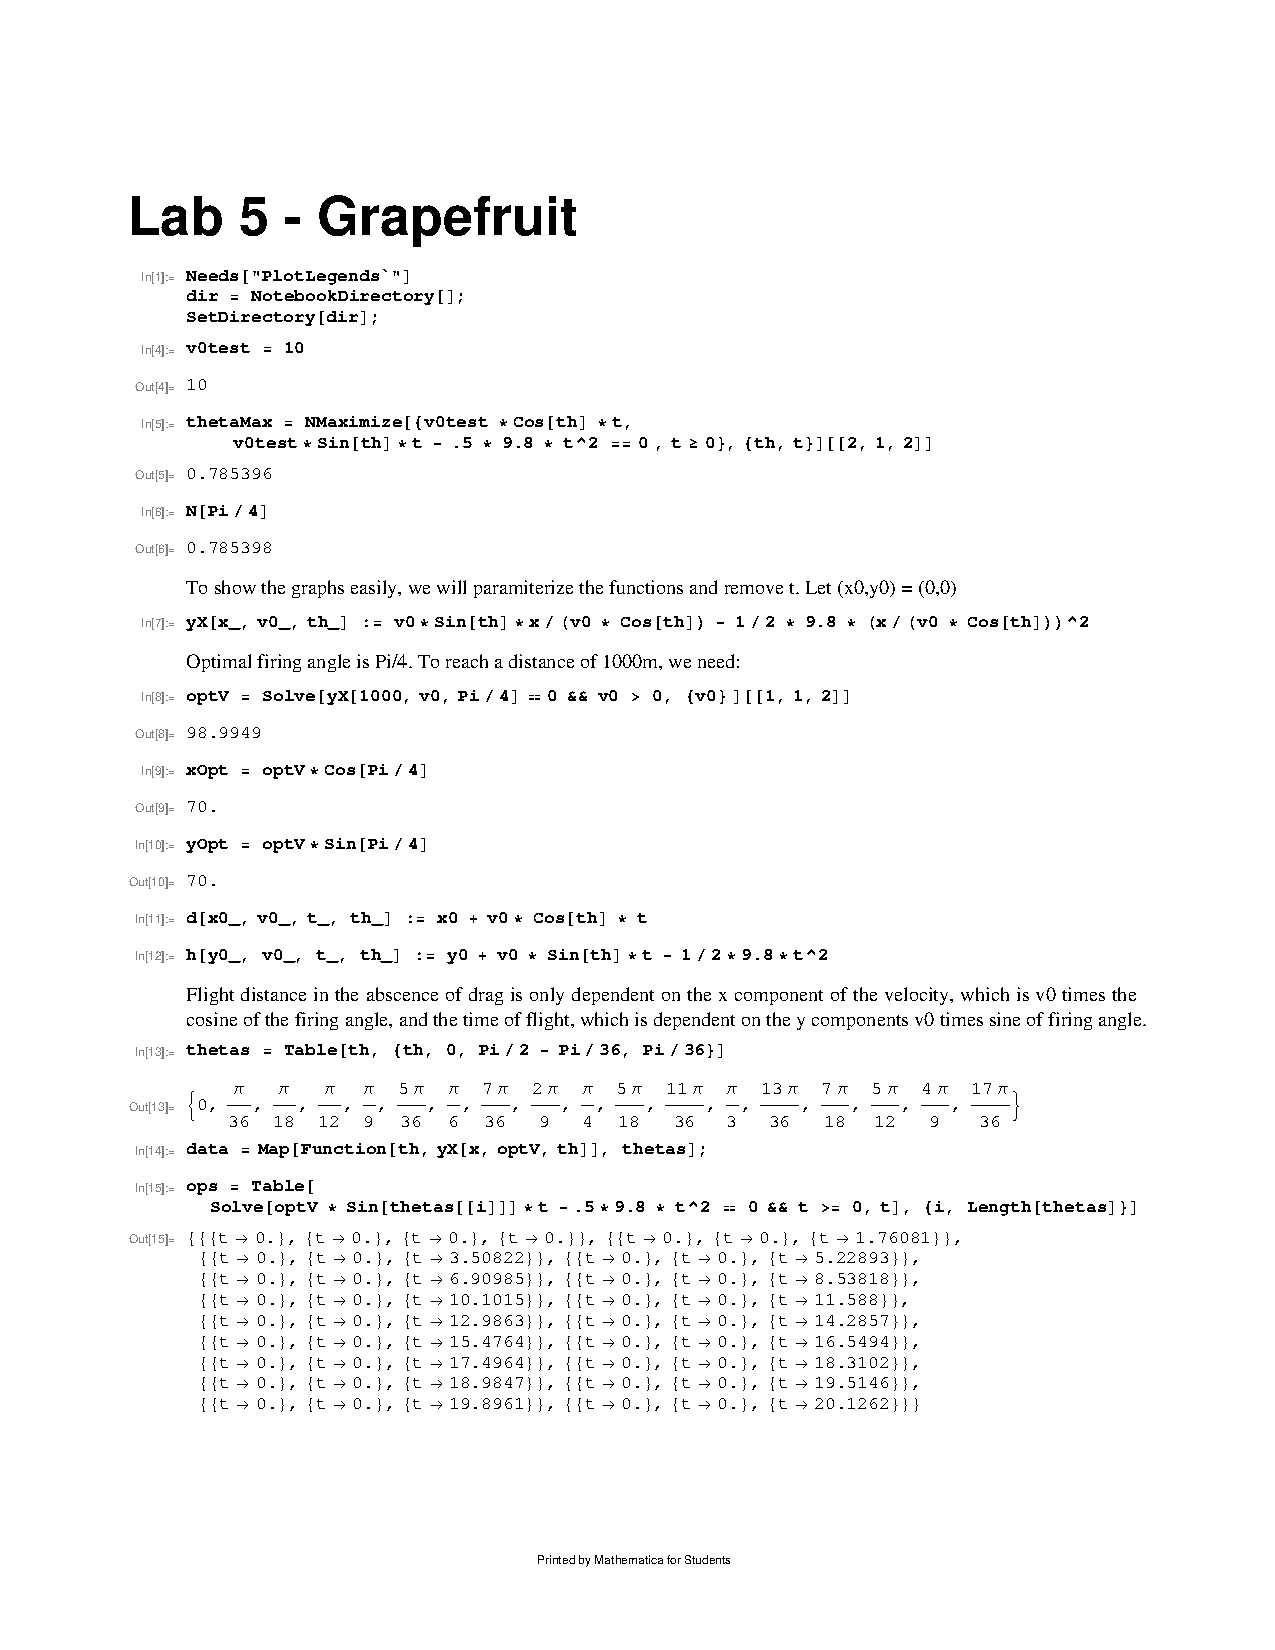
\includepdf[pages={1-10}]{grapefruit.pdf}
\end{document}

\end{document}
